\documentclass[12pt,letterpaper]{article}

\usepackage{graphicx,amssymb,amsmath,bm,color,multicol}
\usepackage{../newcommand}
\sloppy
\newcommand{\ignore}[1]{}

\newenvironment{proof}{\noindent{\bf Proof:}}{\qed\bigskip}

\newtheorem{theorem}{Theorem}
\newtheorem{corollary}{Corollary}
\newtheorem{lemma}{Lemma} 
\newtheorem{claim}{Claim}
\newtheorem{fact}{Fact}
\newtheorem{definition}{Definition}
\newtheorem{assumption}{Assumption}
\newtheorem{observation}{Observation}
\newtheorem{example}{Example}
\newcommand{\qed}{\rule{7pt}{7pt}}

\newcommand{\homework}[4]{
	\thispagestyle{plain} 
	\newpage
	\setcounter{page}{1}
	\noindent
	\begin{center}
		\framebox{ \vbox{ \hbox to 6.28in
				{\bf ECON 4190: Industrial Organization \hfill #1} %change course name
				\vspace{4mm}
				\hbox to 6.28in
				{\hspace{2.5in}\large\mbox{Homework #2}}
				\vspace{4mm}
				\hbox to 6.28in
				{{\it Collaborators: #3\hfill}}
			}}
		\end{center}
	}

\oddsidemargin 0in
\evensidemargin 0in
\textwidth 6.5in
\topmargin -0.5in
\textheight 9.0in

\begin{document}

% Modify this command to be your name and computing ID
\homework{Fall 2021}{$5$}{Alex Shen (as5gd), Sean Velhagen (spv5hq), Max Bresticker (mtb9sex)}

Pledge: On my honor, I pledge that I have neither given nor received help on this assignment 
Signature: \textit{Alex Shen, Sean Velhagen, Max Bresticker}

\begin{enumerate}
	
\item[3.2)] 
\begin{enumerate}
    \item[1.] Note that marginal costs for firms 1 and 2 are $c_1$ and $c_2$ respectively. With that in mind, we maximize their profit functions with respect to quantity (firm 1 work is shown, but by symmetry we solve for both):
    \begin{align*}
        max_{q_1} \pi_1 &= (a - q_1 - q_2 - c_1)q_1 \\
        \frac{\partial \pi_1}{\partial q_1} &= a - 2q_1 - q_2 - c = 0 \\
        q_1 &= \frac{a - q_2 - c_1}{2} \\
        \therefore q_2 &= \frac{a - q_1 - c_2}{2} \\
        \therefore q_1 &= \frac{a - \frac{a - q_1 - c_2}{2} - c_1}{2} \\
        4q_1 &= 2a - a + q_1 + c_2 - 2c_1 \\
        q_1 &= \frac{a + c_2 - 2c_1}{3} \\
        \therefore q_2 &= \frac{a + c_1 - 2c_2}{3}
    \end{align*}  

    Market share can be computed by simply finding $\frac{q_i}{Q}$:
    \begin{align*}
        share_1 &= \frac{a + c_2 - 2c_1}{3} / (\frac{a + c_2 - 2c_1}{3} + \frac{a + c_1 - 2c_2}{3}) \\
        &= \frac{a + c_2 - 2c_1}{3} * \frac{3}{2a - c_1 - c_2} \\
        share_1 &= \frac{a + c_2 - 2c_1}{2a - c_1 - c_2} \\
        share_2 &= 1 - share_1 = \frac{a + c_1 - 2c_2}{2a - c_1 - c_2}
    \end{align*}

    {\color{blue}\textbf{Solution:} $q_1 = \frac{a + c_2 - 2c_1}{3}, q_2 = \frac{a + c_1 - 2c_2}{3}, share_1= \frac{a + c_2 - 2c_1}{2a - c_1 - c_2}, share_2 = \frac{a + c_1 - 2c_2}{2a - c_1 - c_2}$}

    \item[2.] Plug in quantities to determine price and then profits (by symmetry):
    \begin{align*}
        p &= a - q_1 - q_2 = \frac{3a}{3} - \frac{a + c_2 - 2c_1}{3} - \frac{a + c_1 - 2c_2}{3} \\
        p &= \frac{a + c_2 + c_1}{3} \\
        \pi_1 &= (\frac{a + c_2 + c_1}{3} - \frac{3c_1}{3})(\frac{a + c_2 - 2c_1}{3}) \\
        &= (\frac{a + c_2 - 2c_1}{3})^2 = q_1^2\\
        \therefore \pi_2 &= (\frac{a + c_1 - 2c_2}{3})^2 = q_2^2
    \end{align*} 

    Consumer surplus can be measured by finding the definite integral of the demand up to $Q$ (i.e. $q_1 + q_2$), then subtracting the revenue. Graphically, this is the triangle where CS is.

    \begin{align*}
        CS &= \int_0^{q_1 + q_2}[a - Q]dQ - (a - q_1 - q_2)(q_1 + q_2) \\
        &= a(q_1+q_2) - \frac{1}{2}(q_1 + q_2)^2 - (a - q_1 - q_2)(q_1 + q_2) \\
        &= (q_1 + q_2)^2 - \frac{1}{2}(q_1 + q_2)^2 \\
        &= \frac{1}{2}(q_1 + q_2)^2
    \end{align*}
     
    Total welfare can be calculated simply by adding CS and profits:
    \begin{align*}
        W = \frac{1}{2}(q_1 + q_2)^2 + q_1^2 + q_2^2
    \end{align*}

    {\color{blue} \textbf{Solution:} $CS = \frac{1}{2}(q_1 + q_2)^2, PS = q_1^2 + q_2^2, W = \frac{1}{2}(q_1 + q_2)^2 + q_1^2 + q_2^2$}
    \item[3.] Differentiate $W$ with respect to $c_2$:
    \begin{align*}
        W &= \frac{1}{2}(q_1 + q_2)^2 + q_1^2 + q_2^2 \\
        &= \frac{1}{2}(\frac{a + c_2 - 2c_1}{3} + \frac{a + c_1 - 2c_2}{3})^2 + (\frac{a + c_2 - 2c_1}{3})^2 + (\frac{a + c_1 - 2c_2}{3})^2 \\
        &= \frac{1}{2}(\frac{2a - c_1 - c_2}{3})^2 + (\frac{a + c_2 - 2c_1}{3})^2 + (\frac{a + c_1 - 2c_2}{3})^2 \\
        \frac{\partial W}{\partial c_2} &= (\frac{2a - c_1 - c_2}{3})(-\frac{1}{3}) + 2(\frac{a + c_2 - 2c_1}{3})(\frac{1}{3}) + 2(\frac{a + c_1 - 2c_2}{3})(-\frac{2}{3}) \\
        &= (q_1 + q_2)(-\frac{1}{3}) + \frac{2}{3}q_1 - \frac{4}{3}q_2 \\
        &= \frac{1}{3} (-q_1 - q_2 + 2q_1 - 4q_2) = \frac{1}{3}(q_1 - 5q_2) = \frac{1}{3} (q_1 + q_2 - 6q_2) \\
        &= 2 * \frac{1}{6} (q_1 + q_2 - 6q_2) = 2 (q_1 + q_2)(\frac{1}{6} - \frac{q_2}{q_1 + q_2}) \\
        \frac{\partial W}{\partial c_2} &= 2 (q_1 + q_2)(\frac{1}{6} - share_2)
    \end{align*} 

    Thus, if $c_2$ decreases, we know that $W$ will increase when firm 2's market share is greater than $\frac{1}{6}$, and will decrease if market share is less than $\frac{1}{6}$. $\qed$
\end{enumerate} 

\item[4.1)]
\begin{enumerate}
    \item[1.] We start off by maximizing Firm 1's profit:
    \begin{align*}
        max_{p_1} \pi_1 &= (a-2p_1 + p_2)(p_1 - 0) \\
        \frac{\partial \pi_1}{\partial p_1} &= a - 4p_1 + p_2 = 0 \\
        \therefore p_1 &= \frac{a + p_2}{4}
    \end{align*} 
    Then, maximize Firm 2's profit to solve for $p_2$, and then plug in $p_1$ to solve for both:
    \begin{align*}
        max_{p_2} \pi_2 &= (a-2p_2 + p_1)(p_2 - c) \\
        \frac{\partial \pi_2}{\partial p_2} &= (a - 2p_2 + p_1) + (p_2 - c)(-2) = 0 \\
        0 &= a - 2p_2 + p_1 - 2p_2 + 2c \\
        \therefore p_2 &= \frac{p_1 + a + 2c}{4} = \frac{\frac{a + p_2}{4} + a + 2c}{4} \\
        16p_2 &= a + p_2 + 4a + 8c \\
        \therefore p_2 &= \frac{5a + 8c}{15} \\
        \therefore p_1 &= \frac{5 + 2a}{15}
    \end{align*} 

    Solving for profit given these prices is computationally simple, but mostly straightforward:

    \begin{align*}
        \pi_1 &= (\frac{5a+2c}{15})(a - 2 (\frac{5 + 2a}{15}) + \frac{5a + 8c}{15}) \\
        &= (\frac{5a+2c}{15})(\frac{15a}{15} + \frac{-5a + 4c}{15}) \\
        &= (\frac{5a + 2c}{15})(\frac{10a + 4c}{15}) \\
        \pi_1 &= \frac{2}{225}(5a + 2c)^2
    \end{align*}

    \begin{align*}
        \pi_2 &= (\frac{8c + 5a}{15} - c)(a - 2(\frac{8c + 15a}{15} + \frac{5a + 2c}{15})) \\
        &= (\frac{5a - 7c}{15})(\frac{15a}{15} + \frac{-14c - 5a}{15}) \\
        &= (\frac{5a - 7c}{15})(\frac{10a - 14c}{15}) \\
        \pi_2 &= \frac{2}{225}(5a-7c)^2
    \end{align*}

    {\color{blue}\textbf{Solution:} $p_1 = \frac{5 + 2a}{15}, p_2 = \frac{5a + 8c}{15}, \pi_1 = \frac{2}{225}(5a + 2c)^2, \pi_2 = \frac{2}{225}(5a-7c)^2$}
    \item[2.] 
    
    \begin{enumerate}
    
    \item[(a)] Recall that we solved for Firm 2's reaction function, $p_2 = \frac{2c + a + p_1}{4}$. We can then plug this into Firm 1's profit maximization to find $p_1$ (and thus $p_2$ as follows:
    
    \begin{align*}
        max_{p_1} \pi_1 &= p_1 (a - 2p_1 + \frac{2c + a + p_1}{4}) \\
        &= p_1 a - 2p_1^2 + \frac{2cp_1 + ap_1 + p_1^2}{4} \\
        \frac{\partial \pi_1}{\partial p_1} &= a - 4p_1 + \frac{1}{2}c + \frac{1}{4}a + \frac{1}{2}p_1 \\
        \frac{7}{2}p_1 &= \frac{1}{2}c + \frac{5}{4}c \\
        p_1 &= \frac{2c + 5a}{14} \\
        \therefore p_2 &= \frac{2c + a + \frac{2c + 5a}{14}}{4} \\
        &= \frac{28c + 14a + 2c + 5a}{56} \\
        p_2 &= \frac{30c + 19a}{56}
    \end{align*}

    Once again, solving for profit is computationally intensive but quite simple; for levity, only the basic setup and answer are included.

    \begin{align*}
        \pi_1 &= (\frac{2c + 5a}{14})(a - \frac{4c-10a}{14} + \frac{30c + 19a}{56}) = \frac{1}{112}(2c + 5a)^2 \\
        \pi_2 &= (\frac{30c + 19a}{56} -c)(a - 2(\frac{30c + 19a}{56}) + \frac{2c + 5a}{14}) = \frac{1}{1568}(19a - 26c)^2
    \end{align*}

    {\color{blue}\textbf{Solution:} $p_1 = \frac{2c + 5a}{14}, p_2 = \frac{30c + 19a}{56}, \pi_1 = \frac{1}{112}(2c + 5a)^2, \pi_2 = \frac{1}{1568}(19a - 26c)^2$}

    \item[(b)] Recall that we solved for Firm 1's reaction function, $p_1 = \frac{a + p_2}{4}$. Similar to part (a), we plug in that function to Firm 2's profit maximization problem to find prices.
    
    \begin{align*}
        \pi_2 &= (p_2 - c)(a - 2p_2 + \frac{a + p_2}{4}) \\
        &= (p_2 - c)(1.25a - 1.75p_2) \\
        \frac{\partial \pi_2}{\partial p_2} &= -1.75(p_2 - c) + (1.25a - 1.75p_2) = 0 \\
        0 &= -\frac{7}{4} (p_2 -c) + (\frac{5}{4} a - \frac{7}{4} p_2) \\
        &= -\frac{14}{4} p_2 + \frac{7}{4} c + \frac{5}{4} a \\
        p_2 &= \frac{5a + 7c}{14} \\
        \therefore p_1 &= \frac{a + \frac{5a + 7c}{14}}{4} = \frac{19a + 7c}{56}
    \end{align*}

    Once again, for levity we simply plug prices back into the profit equations to get the values.

    \begin{align*}
        \pi_1 &= (\frac{19a + 7c}{56})(a - \frac{38a + 14c}{56} + \frac{20a + 28c}{56}) = \frac{1}{1568}(19a + 7c)^2 \\
        \pi_2 &= \frac{1}{8*14}(5a-7c)^2 = \frac{1}{112}(5a-7c)^2
    \end{align*}

    {\color{blue}\textbf{Solution:} $p_1 = \frac{19a + 7c}{56}, p_2 = \frac{5a + 7c}{14}, \pi_1 = \frac{1}{1568}(19a + 7c)^2, \pi_2 = \frac{1}{112}(5a-7c)^2$}
\end{enumerate}
    \item[3.] For Firm 2 to have a second-mover advantage, its profits as calculated in part (a) must always be greater than part (b). We show that here:
    \begin{align*}
        \frac{1}{1568}(19a - 26c)^2 &> \frac{1}{112}(5a-7c)^2 \\
        \frac{1}{14}(19a - 26c)^2 &> (5a-7c)^2 \\
        (19a - 26c)^2 &> 14 (5a-7c)^2 \\
        19a - 26c &> \sqrt{14}(5a-7c) \\
        19a - 26c &> 5\sqrt{14}a - 7\sqrt{14}c \\
        (19 - 5\sqrt{14})a - (7\sqrt{14}-26)c &> 0
    \end{align*} 

    Since we know that $c<\frac{5}{7}a$, and $c$ can never be negative, this inequality always holds. Therefore, Firm 2 always has a second-mover advantage. $\qed$

    Next, we calculate where Firm 1 has an advantage by also comparing profits - Firm 1 has a first-mover advantage whenever the following inequality holds:
    \begin{align*}
        \frac{1}{112}(2c + 5a)^2 &> \frac{1}{1568}(19a + 7c)^2 \\
        14(2c + 5a)^2 &> (19a + 7c)^2 \\
        2\sqrt{14}c + 5\sqrt{14}a &> 19a + 7c \\
        (2\sqrt{14} - 7)c + (5\sqrt{14} - 19)a &> 0 \\
        (2\sqrt{14} - 7)c &> (19 - 5\sqrt{14})a \\
        c &> \frac{19 - 5\sqrt{14}}{2\sqrt{14}-7} a \\
        c &> 0.604a
    \end{align*}

    Therefore, Firm 1 has a first-mover advantage when $c > 0.604a$. Note that since $c<\frac{5}{7}a$ must also hold, but $\frac{5}{7} \approx 0.714$ so this is fine. $\qed$
\end{enumerate}

\item[4.3)] 

\begin{enumerate}
    \item[1.] The game tree here can be (roughly) visualized as follows:

    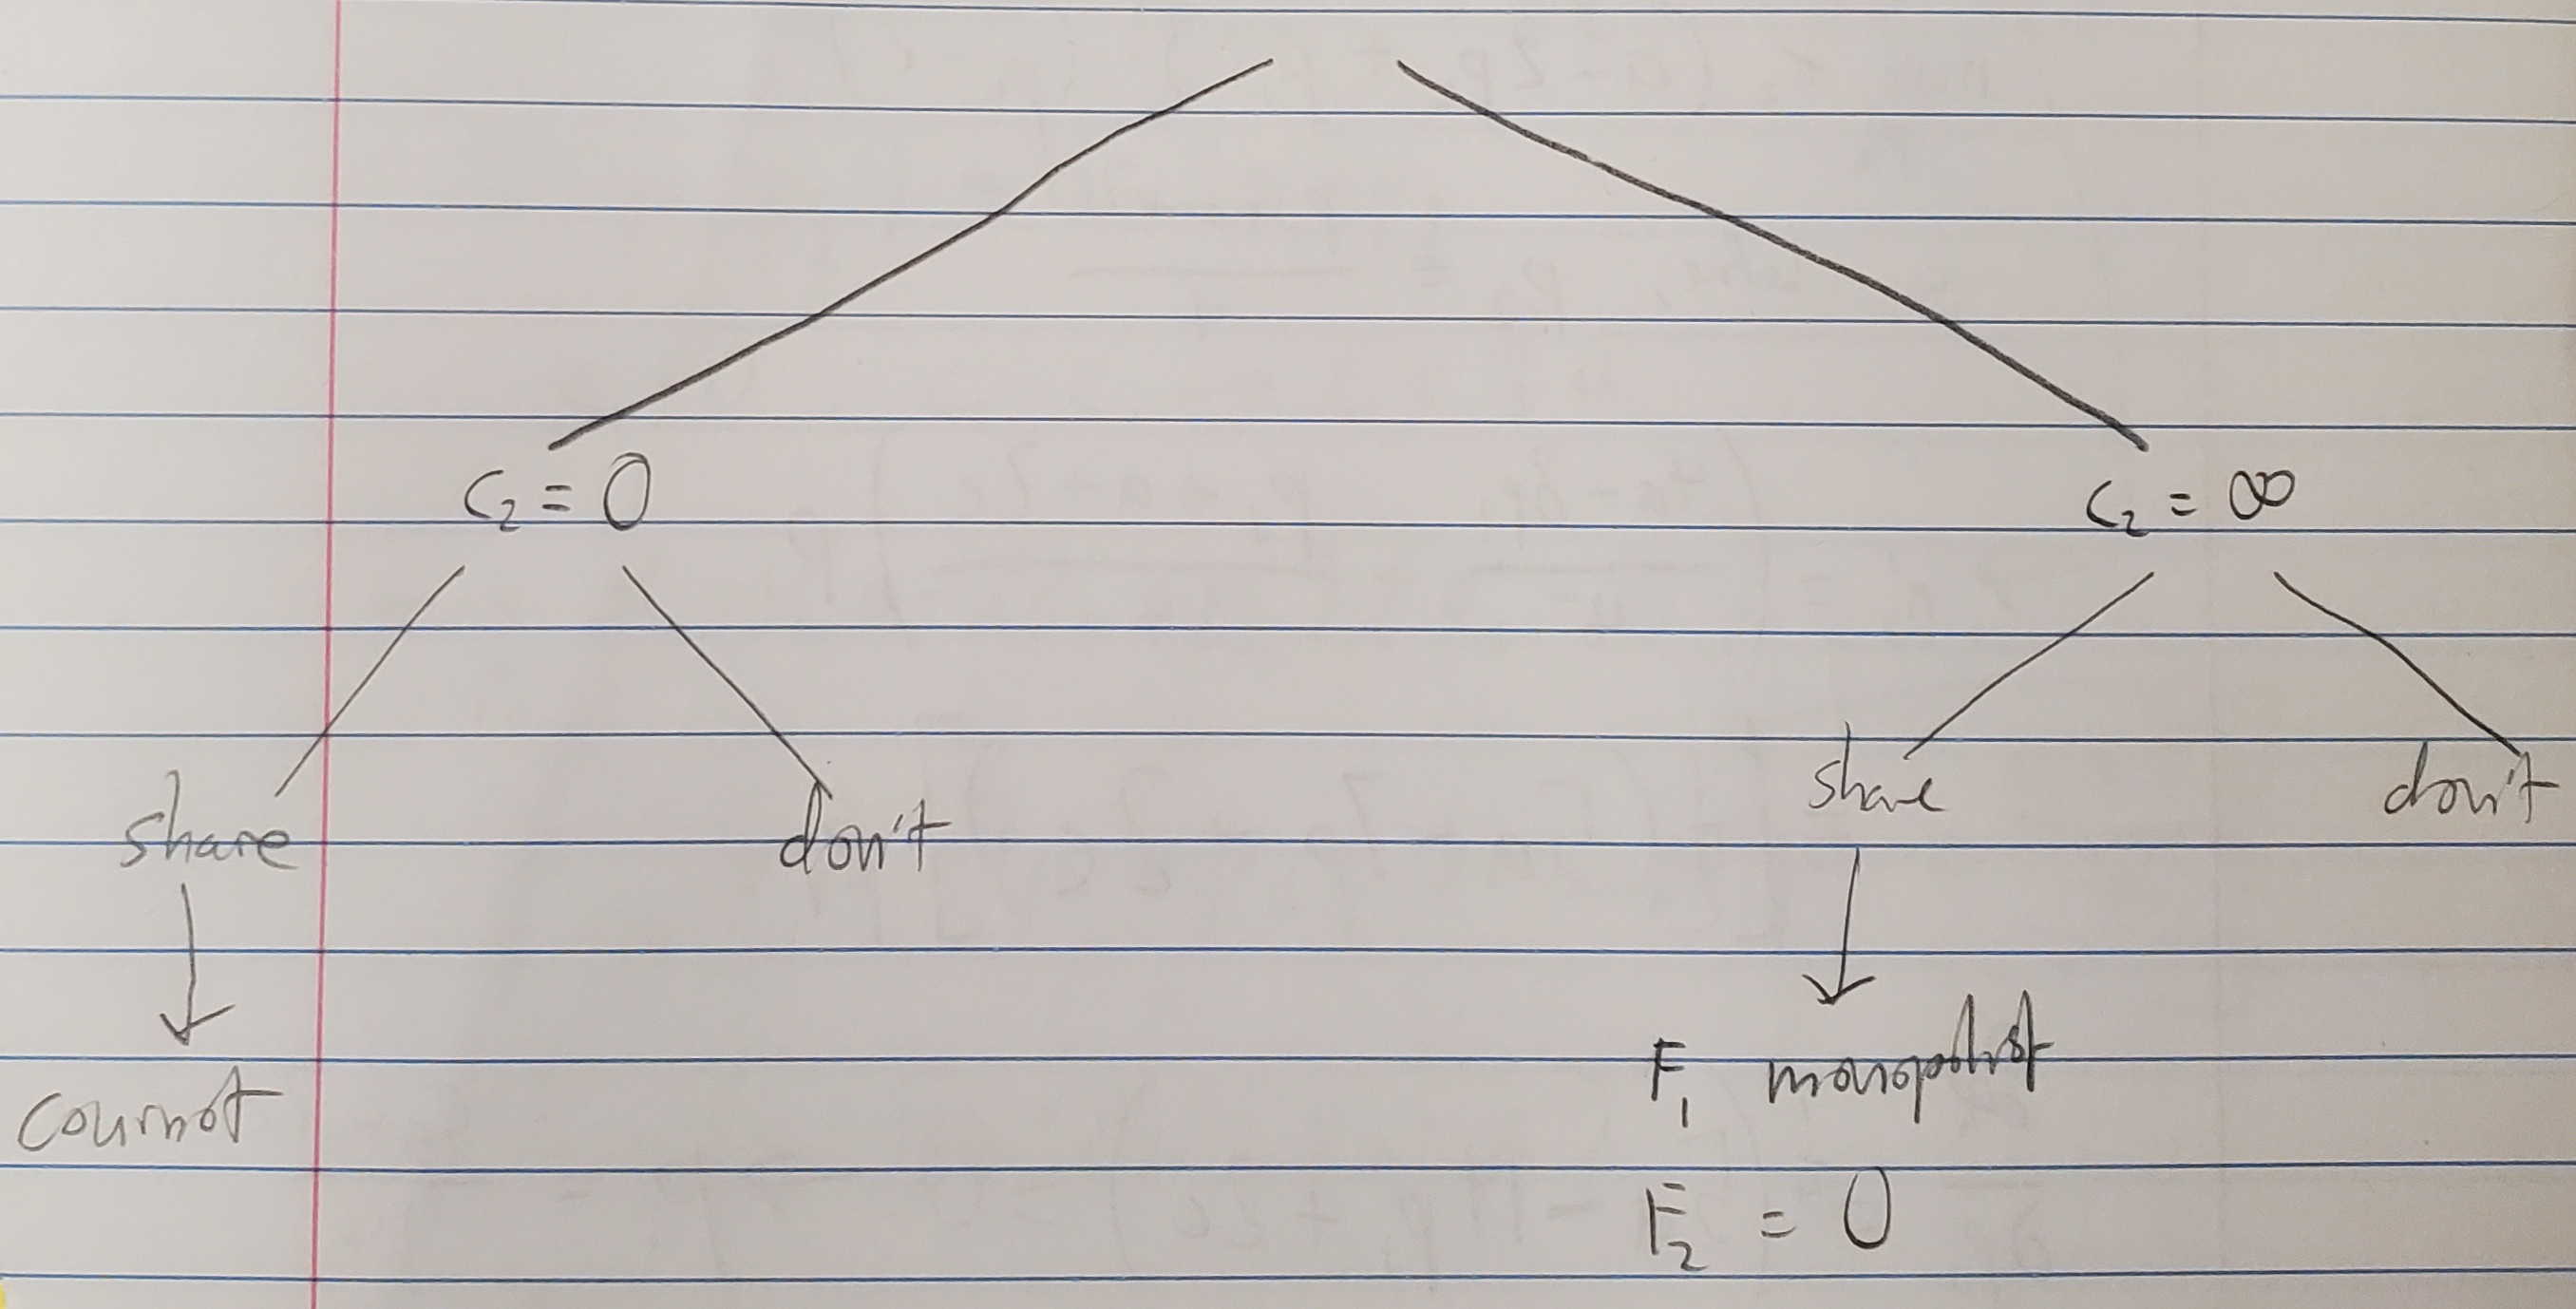
\includegraphics[scale=0.15]{game-tree.jpg}
                                          
    In scenarios where Firm 2 discloses its cost, Firm 1's response is very simple - when $c_2 = 0$, the firms have equal costs and will thus reach the Cournot equilibrium outcome, where $q_1 = q_2 = \frac{1}{3}$, and $\pi_1 = \pi_2 = (1-q -q)* q= \frac{1}{9}$. If $c_2$ is prohibitively high, then Firm 1 will simply act as a monopolist, producing $q=\frac{1}{2}$ with a profit of $\frac{1}{4}$, whereas Firm 2 will have a quantity produced and profit of 0.
    
    When Firm 2 doesn't disclose its cost, Firm 1 can only maximize its profit function using an expected value for $q_2$. Since the probability of both cases is $p=0.5$, $E(p_2)$ can be determined simply by halving the quantity Firm 2 produces in the Cournot equilibrium, so $E(q_2) = \frac{1-q_1}{2} * \frac{1}{2} = \frac{1-q_1}{4}$. Given this value, we can simply derive Firm 1's best response as follows by maximizing their expected profit:
    
    \begin{align*}
        max_{q_1} E(\pi_1) &= (1 - q_1 - E(q_2)) * (q_1) \\
        \frac{\partial E(\pi_1)}{\partial q_1} &= 1 - 2q_1 - E(q_2) = 0 \\
        \therefore q_1^* &= \frac{1 - E(q_2)}{2} \\
        &= \frac{1}{2} * (1 - \frac{1-q_1}{4}) \\
        8q_1 &= 4 - 1 + q_1 \\
        q_1 &= \frac{3}{7} \\
        \therefore q_2 &= \frac{2}{7}
    \end{align*}
    
    With these quantities, we can easily determine the profits to be $\pi_1 = (1 - \frac{3}{7} - \frac{2}{2*7}) * \frac{3}{7} = \frac{9}{49}$ (plugging back into our expected value function) and $\pi_2 = (1 - \frac{3}{7} - \frac{2}{7}) * \frac{2}{7} = \frac{4}{49}$ (since Firm 1 is always in the market, Firm 2 doesn't need to use expected values).
    
    {\color{blue}\textbf{Solution:} With information sharing, the outcome will either resemble that of Cournot duopoly if $c_2=0$ or monopoly by Firm 1 if $c_2$ is prohibitively high. Without information sharing, the equilibrium is $q_1  = \frac{3}{7}, q_2 = \frac{2}{7}, \pi_1 = \frac{9}{49}, \pi_2 = \frac{4}{49}$}

    \item[2.] If $c_2$ is prohibitively high, then Firm 2 doesn't care about sharing its information because its profit is 0 either way. Otherwise, if $c_2 = 0$, Firm 2 has an incentive to share its cost as $\frac{1}{9} > \frac{4}{49}$ i.e. their profit is higher in the Cournot duopoly equilibrium than the non-sharing equilibrium. 
    \item[3.] If Firm 2 shares information, then Firm 1's expected profit is $\frac{1}{2} (\frac{1}{4} + \frac{1}{9}) = \frac{13}{72}$. This is less than the expected profit of $\frac{9}{49}$s when information is not shared, so Firm 1 is worse off in information sharing.
\end{enumerate}

\item[4)]

\begin{enumerate}

    \item In general, the profit function for a monopoly (colluding firms) is as follows:
    \begin{align*}
        \pi^m &= P(Q)Q - c(Q)
    \end{align*}
    
    In this case, $P(Q) = a-bQ$ and $c(Q) = cQ$, so:
    \begin{align*}
        \pi^m &= (a-bQ)Q - cQ\\
        FOC_{wrt.Q}: 0 &= a-2bQ^m - c\\
        Q^m &= \frac{a-c}{2b}
    \end{align*}
    
    Firm i's profit function in a 2-firm Cournot model with the given inverse demand and cost function is as follows:
    \begin{align*}
        \pi_i &= (a - b(q_1 + q_2))q_i - cq_i
    \end{align*}
    
    So, the firms' profit functions are as follows:
    \begin{align*}
        \pi_1 &= (a - b(q_1 + q_2))q_1 - cq_1\\
        \pi_2 &= (a - b(q_1 + q_2))q_2 - cq_2
    \end{align*}
    
    It is easily seen here that optimizing firm 1's profits will give a similar expression to optimizing firm 2's profits, just with $q_1$ and $q_2$ interchanged. Let us optimize firm 1:
    \begin{align*}
        FOC_{wrt.q_1}: 0 &= -bq_1^c + (a-b(q_1^c + q_2)) - c\\
        0 &= a - 2bq_1^c - bq_2 - c\\
        q_1^c &= \frac{a - bq_2 - c}{2b}
    \end{align*}
    
    We may interchange $q_1$ and $q_2$ to find $q_2^c$:
    \begin{align*}
        q_2^c &= \frac{a - bq_1 - c}{2b}
    \end{align*}
    
    To find the Cournot equilibrium, we can plug in firm 2's best response  function into firm 1's best response function and solve for $q_1^c$ as a function of constants. Again, we see here that the process for solving for $q_1^c$ as a function of constants is similar to the process for solving for $q_2^c$ as a function of constants, just with $q_1^c$ and $q_2^c$ flipped. Plugging $q_2^c$ into firm 1's best response function, we have:
    \begin{align*}
        q_1^c &= \frac{a - b(\frac{a - bq_1^c - c}{2b}) - c}{2b}\\
        q_1^c &= \frac{a}{2b} - \frac{a}{4b} + \frac{q_1^c}{4} + \frac{c}{4b} - \frac{c}{2b}\\
        \frac{3}{4}q_1^c &= \frac{a}{4b} - \frac{c}{4b}\\
        q_1^c &= \frac{a-c}{3b}
    \end{align*}
    
    We may interchange $q_1^c$ and $q_2^c$ to find $q_2^c$ as a function of constants:
    \begin{align*}
        q_2^c &= \frac{a-c}{3b}\\
        Q &= q_1 + q_2\\
        Q^c &= q_1^c + q_2^c\\
        Q^c &= \frac{2(a-c)}{3b}\\
        Q^m &= \frac{a-c}{2b}\\
        \frac{2(a-c)}{3b} &> \frac{a-c}{2b}\\
        Q^c &> Q^m \ \blacksquare
    \end{align*}
    
    \item As previously solved for in part 4.a, firm i's profit under a Cournot system is $\pi_i = (a-b(\frac{2(a-c)}{3b}))(\frac{(a-c)}{3b}) - c(\frac{(a-c)}{3b}) = \frac{1}{9b}(a-c)^2$. For both firms to choose to collude, they would each need profits equal to or exceeding what they would have gotten had they competed under a Cournot system. Given that each firm is colluding, they would collectively produce the monopoly quantity: $Q^m$. If firms cannot freely transfer profits, then each firm must produce a quantity that satisfies their respective profit condition.
    
    \item $MC(q_i) = cq_i$, so the profit function for firm i is as follows:
    \begin{align*}
        \pi_i &= (a - b(q_1 + q_2))q_i - \frac{cq_i^2}{2}
    \end{align*}
    
    We can find $q_1^c$ and $q_2^c$ using the same techniques that we used in 4.a:
    \begin{align*}
        \pi_1 &= (a - b(q_1 + q_2))q_1 - \frac{cq_1^2}{2}\\
        FOC_{wrt.q_1}: 0 &= -bq_1^c + (a-b(q_1^c + q_2)) - cq_1^c\\
        0 &= a - (2b + c)q_1^c - bq_2\\
        q_1^c &= \frac{a - bq_2}{2b + c}
    \end{align*}
    
    By symmetry, we have:
    \begin{align*}
        q_2^c &= \frac{a - bq_1^c}{2b + c}
    \end{align*}
    
    Again, we plug $q_2^c$ into $q_1^c$ to get $q_1^c$ as a function of constants:
    \begin{align*}
        q_1^c &= \frac{a - b(\frac{a - bq_1^c}{2b + c})}{2b + c}\\
        q_1^c &= \frac{a}{2b+c} - \frac{ab}{(2b+c)^2} + \frac{b^2q_1^c}{(2b+c)^2}\\
        (1-\frac{b^2}{(2b+c)^2})q_1^c &= \frac{a(b+c)}{(2b+c)^2}\\
        ((2b+c)^2 - b^2)q_1^c &= a(b+c)\\
        q_1^c &= \frac{a(b+c)}{3b^2 + 4bc + c^2}
    \end{align*}
    
    By symmetry, we have:
    \begin{align*}
        q_2^c &= \frac{a(b+c)}{3b^2 + 4bc + c^2}\\
        Q^c &= q_1^c + q_2^c\\
        \therefore Q^c &= \frac{2a(b+c)}{3b^2 + 4bc + c^2}
    \end{align*}
    
    \item If the firms do not have to worry about getting caught, then the firms should simply have the firm with the lower marginal cost produce all of the quantity and have the lower-cost firm transfer an amount of profit equal to or greater than the other firm's profit under a Cournot system. This is to give the other firm an incentive to collude. If, instead, the firms do have to worry about getting caught (and, therefore, cannot transfer profits), then each firm would have to act like they're still competing in some capacity. Therefore, each firm must produce a quantity such that their respective profits are higher than they would be under a Cournot system, similarly to 4.b.

\end{enumerate}


\end{enumerate}
	
\end{document}
